\usetikzlibrary{arrows.meta,calc,matrix}

\begin{frame}{Linux x86-64 calling convention}
    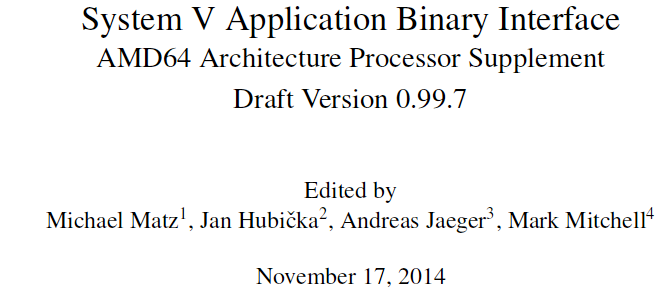
\includegraphics[width=\textwidth]{../asm/sysv-abi-front}
\end{frame}

\begin{frame}{Linux x86-64 calling summary}
\begin{itemize}
    \item first 6 arguments: \%rdi, \%rsi, \%rdx, \%rcx, \%r8, \%r9
    \item additional arguments: push on stack
    \item return address: push on stack
        \begin{itemize}
        \item {\tt call}, {\tt ret} instructions assume this
        \end{itemize}
    \item return value: \%rax
\end{itemize}
\end{frame}

\begin{frame}{caller-saved registers}
    \begin{itemize}
        \item functions \myemph{may} freely \myemph{trash} these
        \vspace{.5cm}
        \item return value register {\tt \%rax}
        \item argument registers: \\
            \begin{itemize}
            \item {\tt \%rdi}, {\tt \%rsi}, {\tt \%rdx}, 
              {\tt \%rcx}, {\tt \%r8}, {\tt \%r9}
              \end{itemize}
        \item \%r11
        \item MMX/SSE/AVX registers: {\tt \%xmm0-15}, etc.
        \item floating point stack: {\tt \%st(0)-\%st(7)}
        \item condition codes (used by {\tt jne}, etc.)
    \end{itemize}
\end{frame}

\begin{frame}[fragile,label=calleeSaved]{callee-saved registers}
    \begin{itemize}
    \item functions \myemph{must preserve} these
    \vspace{.5cm}
    \item {\tt \%rsp} (stack pointer), {\tt \%rbp} (frame pointer, maybe)
    \item {\tt \%r12-\%r15}
    \end{itemize}
\end{frame}

\begin{frame}[fragile,label=callerCallee]{caller/callee-saved}
\lstset{style=small}
\begin{lstlisting}
foo:
    pushq %r12 // r12 is caller-saved
    ... use r12 ...
    popq %r12
    ret

...
other_function:
    pushq %r11 // r11 is caller-saved
    ...
    callq foo
    popq %r11
\end{lstlisting}
\end{frame}

% XXX enter/leave ???

\subsection{the call stack}

\begin{frame}[fragile,label=callStack]{the call stack}
\begin{lstlisting}[language=C,style=small]
foo(a,b,c,d,e,f,g,h);
\end{lstlisting}
\begin{tikzpicture}
\tikzset{>=Latex}
\matrix[tight matrix,nodes={text width=7cm,font=\tt}] (theStack) {
    \ldots \\
    \normalfont (stack allocations in caller) \\
    \normalfont (saved registers, if any) \\
    h \\
    g \\
    \normalfont return address \\
    \normalfont (first stack allocation in {\tt foo}) \\
    \ldots \\
};
\draw[very thick,->] ([xshift=0.25cm]theStack-1-1.east)  -- ([xshift=0.25cm]theStack-8-1.east)
    node[right] {decreasing addresses};
\draw[red,thick,->] (theStack-6-1.east) -- ++(.5cm,0cm) node[right] {stack pointer after call};
\end{tikzpicture}
\end{frame}

\begin{frame}[fragile,label=conventionEx]{calling convention example}
\begin{lstlisting}[language=C,style=small]
int foo(int a, int b, int c, int d, int e, int f, int g, int h);
...
foo(1, 2, 3, 4, 5, 6, 7, 8);
\end{lstlisting}
\begin{lstlisting}[language=myasm,style=small]
pushq   $8
pushq   $7
movl    $6, %r9d
movl    $5, %r8d
movl    $4, %ecx
movl    $3, %edx
movl    $2, %esi
movl    $1, %edi
call    foo
/* return value in %eax */
\end{lstlisting}
\end{frame}

